\chapter{\centering General context and preliminary study}

\section{Introduction}
This chapter will explain where our project fits.
We begin with the Project framework, presenting the host company,
KTS (Kabelbaum Test Systems). Next, we make a study of the existing Process 
to address the problem that caused the host organization to develop this platform.
We evaluate existing solutions to identify where they lack the company's needs and propose the direction of our solution.
Finally, we present the methodology used for the development of our project.

\section{Project Framework}
This project was carried out as part of a final year project submitted
to the Faculty of Sciences of Monastir for the award of a Bachelor's degree in Software Engineering and Information Systems. I worked at the company "KTS" for three months to design and develop a production tracking platform that helps the company to manage its production flow and inventory more efficiently.

\section{Presentation of the Host Organization}

KTS Kabelbaum Test Systems is a company established in 2019 in Bursa, Turkey, operating within a 2,000 m² indoor facility. The company was founded with the objective of meeting the needs of wiring harness manufacturers by providing specialized solutions and acting as a reliable solution partner in the industry\hyperref[ref:KTSintro]{[2]}.
\begin{figure}[h]
    \centering
    
\includegraphics[width=6cm]{pictures/logo (1).png}
    \caption{Host organisation KTS logo  \hyperref[ref:KTSlogo]{[3]}}
    \label{fig:host-organisation-logo}
\end{figure}

KTS expanded to Tunisia in 2025 , all general information about the company is summerised in the table below:
\begin{table}[H]
    
    \begin{tabular}{|>{\raggedright\arraybackslash}p{4cm}|>{\raggedright\arraybackslash}p{10cm}|}
        \hline
        \textbf{Company Name} & KTS (Kabelbaum Test Systems) \\
        \hline
        \textbf{Founded} & 2025 \\
        \hline
        \textbf{Location} & 1 ZI Mghira, 65 Rue Khlidia, Ben Arous, Tunisia, 2082 \\
        \hline
        \textbf{Industry} & Industrial Automation, Manufacturing Solutions \\
        \hline
        \textbf{Phone number} & +216 57 030 790 \\
        \hline
        \textbf{Website} & \url{https://www.ktsistem.com} \\
        \hline
        \textbf{E-mail} & \url{info-tn@ktsistem.tn} \\
        \hline
        \textbf{Director} & Mehrez Ayadi \\
        \hline
    \end{tabular}
    \caption{General Information about KTS}
\end{table}





\section{Study of Existing Processes}

\subsection{Description of Current State}

Production tracking at KTS currently operates through a paper-based workflow.
where Work orders are created by the Sales department and circulate physically through all eight production stages.
At each stage, workers manually update progress, documente completion of tasks, resource allocation, and readiness for the next phase.
Inventory management is similarly manual where workers check physical stock records and update them by hand when materials are reserved or consumed.
Communication between stages relies on direct contact and physical documentation,
with no centralized system to track production progress or resource availability.

\subsection{Critique of Existing System}

The current paper-based system shows several limitations:

\begin{itemize}
    \item \textbf{Lack of Traceability:} Information is divided across multiple physical documents, making it difficult to track the complete history of a work order's progression.
    \item \textbf{Communication Delays:} Physical communication between stages introduces delays and creates bottlenecks in the production workflow.
    \item \textbf{Visibility limitations:} Management has limited visibility into production status, and inventory levels.
    \item \textbf{Error Prone:} Manual data entry and documentation increases the risk of errors .
    \item \textbf{Scalability Issues:} As production volume increases, the manual system becomes increasingly difficult to manage.
\end{itemize}

the paper-based system is easy to use and has a low cost, but unfortunately, these aspects no longer satisfies the company’s purposes.
\subsection{Existing Solutions}
\subsubsection{SMOFT ERP}
SMOFT ERP is a cloud-based enterprise resource planning platform that provides a modular set of business applications for managing operations across different departments. It focuses on centralizing information, supporting configurable workflows, and giving companies a unified environment for data management and process coordination\hyperref[ref:SMOFT]{[4]}.

\begin{itemize}
    \item \textbf{Integrated business management:} Brings several operational functions into one platform.
    \item \textbf{Modular structure:} Can be adapted according to company needs and growth.
    \item \textbf{Centralized data:} Reduces information fragmentation across departments.
\end{itemize}

\textbf{Weak points:}
\begin{itemize}
    \item It is mainly ERP-oriented, so it is not specialized for detailed shop-floor execution.
    \item Production-stage visibility and operator-level tracking are not the main focus.
    \item It can be broader than what a mid-sized manufacturing company needs for a dedicated production tracking workflow.
\end{itemize}

\begin{figure}[h]
    \centering
    
\includegraphics[width=4cm]{pictures/SMOFT-LOGO.png}
    \caption{SMOFT official logo \hyperref[ref:SMOFT-LOGO]{[5]}}
    \label{fig:smoft-logo}
\end{figure}

\begin{figure}[h]
    \centering
    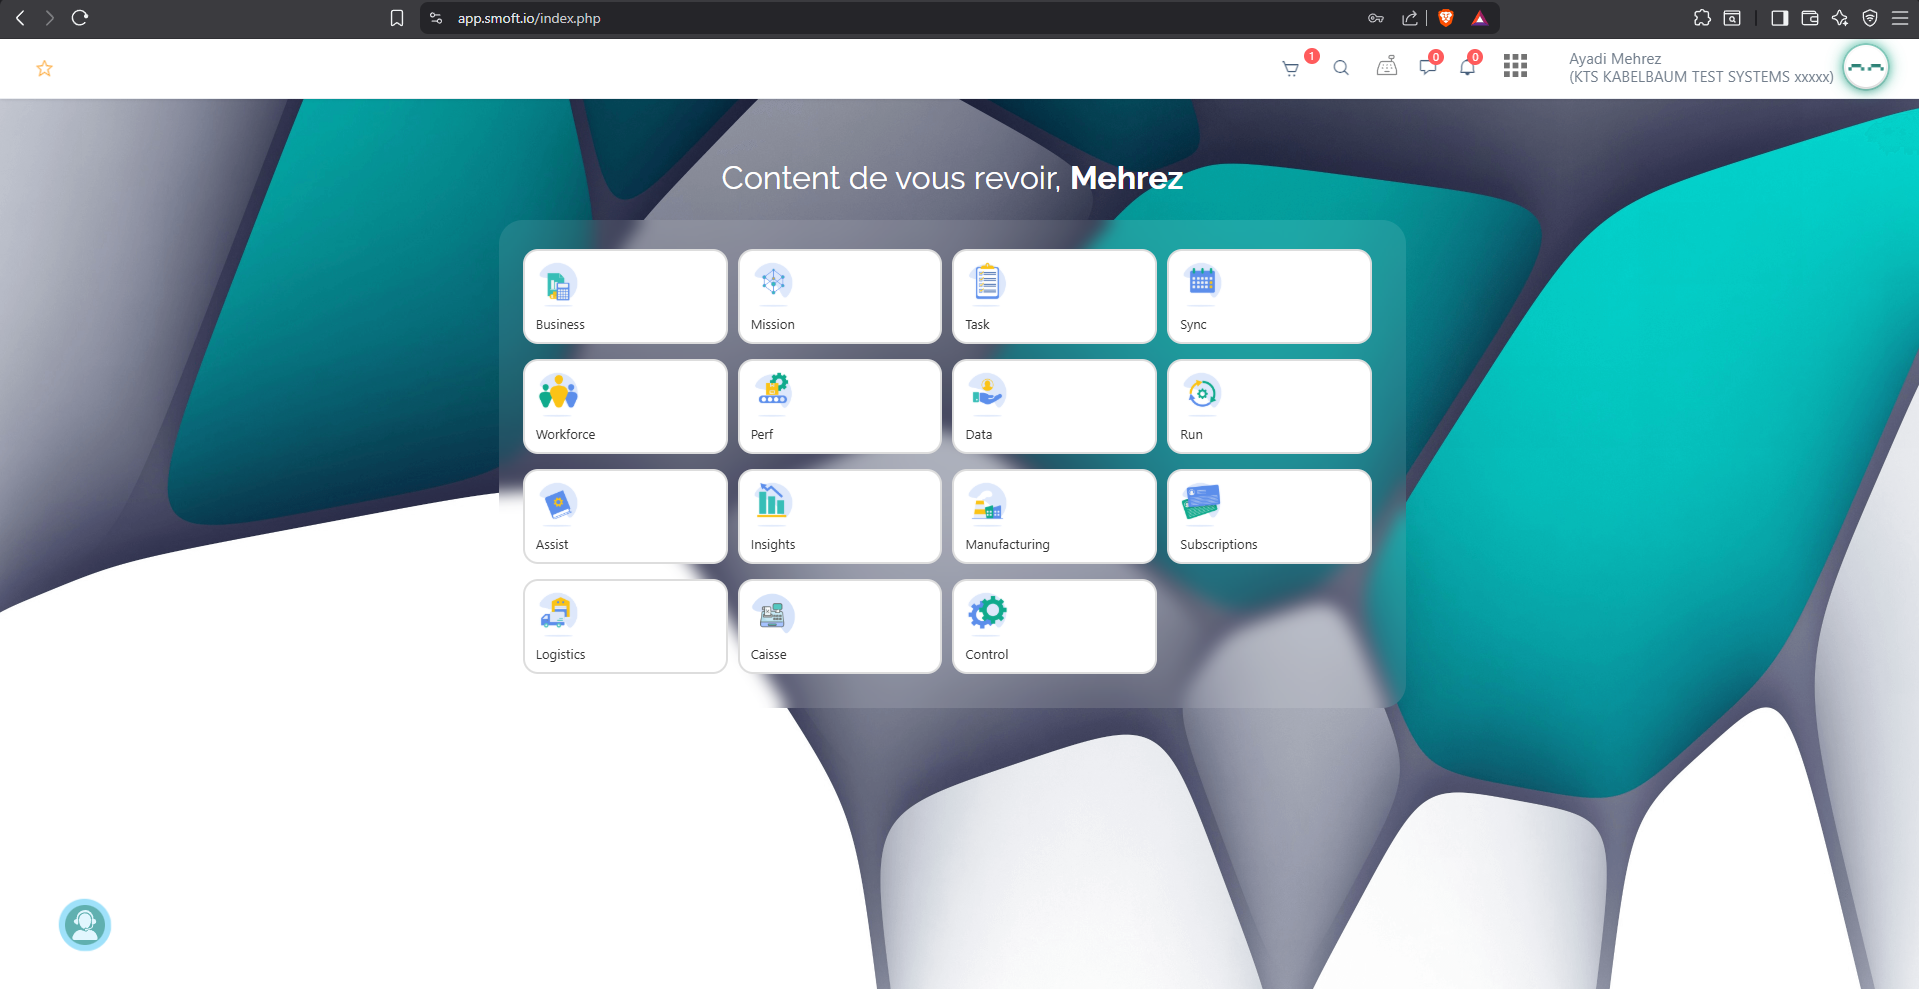
\includegraphics[width=12cm]{pictures/smoft-dashboard.png}
    \caption{SMOFT dashboard }
    \label{fig:smoft-dashboard}
\end{figure}
\subsubsection{SAP Digital Manufacturing}
SAP Digital Manufacturing is SAP's manufacturing execution and operations management solution. It connects shop-floor activities with enterprise planning, supports real-time production visibility, and helps manufacturing teams coordinate execution, traceability, and performance monitoring\hyperref[ref:SAPDM]{[6]}.

\begin{itemize}
    \item \textbf{Shop-floor coordination:} Supports execution of production activities directly from the manufacturing floor.
    \item \textbf{Real-time visibility:} Gives managers current information about ongoing production.
    \item \textbf{Traceability support:} Helps track production progress and operational events.
\end{itemize}

\textbf{Weak points:}
\begin{itemize}
    \item Deployment and integration can be complex for a small or medium company.
    \item The solution may require significant configuration and user training.
    \item It can be more expensive and heavier than a focused platform built for KTS-specific needs.
\end{itemize}

\begin{figure}[H]
    \centering
    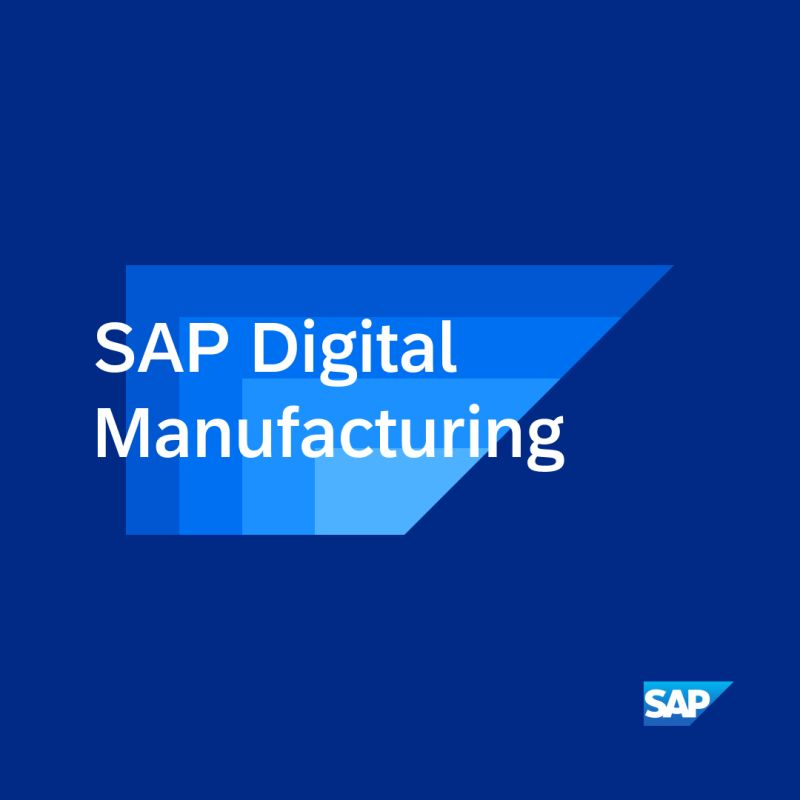
\includegraphics[width=4cm]{pictures/SAP DigitalManufacturing Logo.jpg}
    \caption{SAP Digital Manufacturing  \hyperref[ref:SAPDM-LOGO]{[7]}}
    \label{fig:sap-logo}
\end{figure}

\begin{figure}[h]
    \centering
    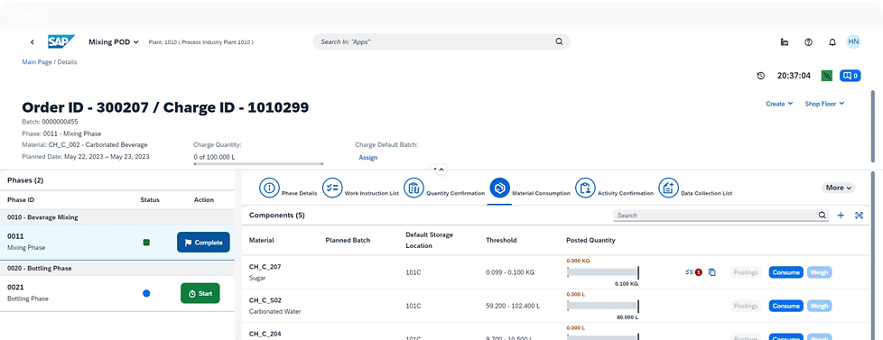
\includegraphics[width=12cm]{pictures/sap-dashboard.png}
    \caption{SAP Digital Manufacturing dashboard \hyperref[ref:SAPDM-DASHBOARD]{[8]}}
    \label{fig:sap-dashboard}
\end{figure}
\subsection{Proposed Solution}

Two alternatives were considered:

\subsubsection*{Alternative 1: degital logbook system}
Deploy a simple digital logbook system to replace paper forms while maintaining existing workflows. This approach minimizes disorder but can't improve processes that much.

\subsubsection*{Alternative 2:Production Management Platform}
Develop a web-based application that standardizes workflows,
offers role-based access control,
provides real-time production visibility,
and integrates inventory management.


\vspace{0.5cm}


The chosen approach is Alternative 2,
a comprehensive platform,
because it addresses not only the paper based process but also provide other solutions for better production managment. The implementation includes:

\begin{itemize}
    \item \textbf{centralized Tracking:} A unified platform where all work orders and tasks are digitally recorded.
    \item \textbf{Real-Time Visibility:} Administrators and workers access current status immediately, reducing communication delays.
    \item \textbf{Role-Based access:} Tailored interfaces and permissions for administrators, production workers.
    \item \textbf{Integrated inventory:} Stock management features linked directly to work orders, with reservation updates.
    \item \textbf{Chat messaging:} communication tool for better visibility and understanding.
    \item \textbf{Scalability:} A web-based architecture that grows with the company's production volume without the increase of manual efforts.
\end{itemize}
This solution is the best approache cause it solves a lot of linmitations and helps the company to grow efficiently.

The table \ref{tab:comparison} summarizes the comparison between the existing solutions and our project:
\begin{table}[H]
    \centering
    \caption{Comparison of Existing Solutions with Our Project} \label{tab:comparison}
    \renewcommand{\arraystretch}{1.2}
    \small
    \begin{tabularx}{\textwidth}{|p{3.6cm}|>{\raggedright\arraybackslash}X|>{\raggedright\arraybackslash}X|>{\raggedright\arraybackslash}X|}
        \hline
        \textbf{Criterion} & \textbf{SMOFT ERP} & \textbf{SAP Digital Manufacturing} & \textbf{Our project} \\
        \hline
        Traceability & Basic transactional traceability across business modules. & Strong production traceability for shop-floor operations. & Full traceability from work orders to stages, stock, notes, and chat. \\
        \hline
        Real-time visibility & Limited to ERP-level monitoring. & Good real-time production visibility. & Real-time visibility across production stages and inventory. \\
        \hline
        Role-based access & Available at business level, but not tailored to production roles. & Supports structured access for manufacturing users. & Dedicated access for administrators and production workers. \\
        \hline
        Usability for KTS & Too general for a dedicated production tracking workflow. & Powerful but heavier than required. & Designed specifically for KTS production tracking needs. \\
        \hline
        Deployment effort & Moderate, depending on customization. & High integration and configuration effort. & Lower effort because it is focused on the exact workflow. \\
        \hline
        Fit for KTS & Partial fit. & Partial fit, but more complex than necessary. & Best fit because it matches the company's process and constraints. \\
        \hline
    \end{tabularx}
\end{table}



\section{Work Methodology}

\subsection{Agile Scrum Method}

\hyperref[ref:scrumguide]{[9]} Scrum is a lightweight framework that helps people,
 teams and organizations generate value through adaptive solutions for complex problems.

In a nutshell, Scrum requires a Scrum Master to foster an environment where:

\begin{itemize}
    \item \textbf{1-} A Product Owner orders the work for a complex problem into a Product Backlog
    \item \textbf{2-} The Scrum Team turns a selection of the work into an Increment of value during a Sprint.
    \item \textbf{3-} The Scrum Team and its stakeholders inspect the results and adjust for the next Sprint.
    \item \textbf{4-} Repeat
\end{itemize}
During this project, \textbf{ Mr. Ayadi Mahrez} served as the Product Owner and Scrum Master to ensure that there was supervision in the project, prioritization of requirements, and management of the Scrum process. The members of the Scrum Team comprised only me as the developer of the application


\begin{figure}[H]
    \centering
    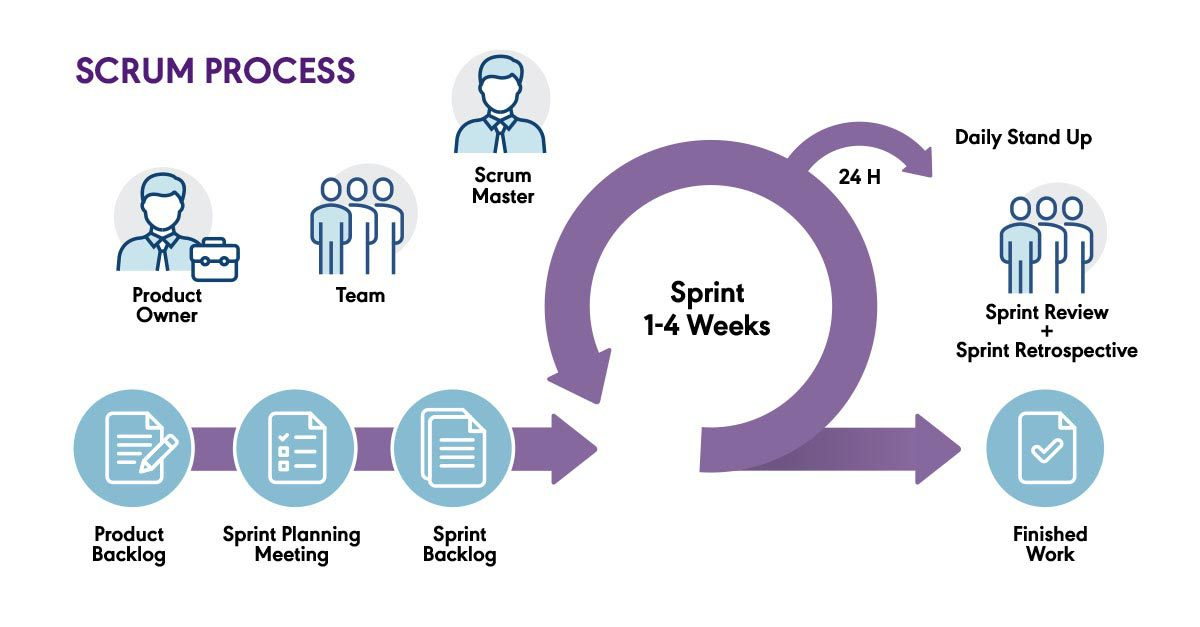
\includegraphics[width=12cm]{pictures/Scrum-methodology.jpg}
    \caption{SCRUM Process \hyperref[ref:scrum-Process]{[10]}}
    \label{fig:scrum-method}
\end{figure}

\section{Methodology: Scrum Sprint Summary}

Five sprints were carried out using the Scrum methodology to implement a usable increment of the production Tracker platform in each step.
The table \ref{tab:sprint-summary} summarizes the objectives and goals of each sprint.

\begin{table}[H]
    \caption{Task by Scrum Sprint} \label{tab:sprint-summary}
    \begin{tabular}{|p{1.5cm}|p{5.5cm}|p{7cm}|}
        \hline
        \textbf{Sprint} & \textbf{Objective} & \textbf{Goals} \\
        \hline
        1 & Foundation and Access \newline Control &  Establish authentication, \newline authorization, and a stable user management foundation\\
        \hline
        2 & Work Orders and Stage \newline Tracking & Enable the core production workflow from work order creation to stage history. \\
        \hline
        3 & Stock Management & Deliver a usable stock management system with validation and reliable inventory rules along with reservation functionality.\\
        \hline
        4 & Notes, Real-Time Chat,  and Notifications & Improve traceability and keep users informed in real time using communication and notification tools \\
        \hline
        5 & QR Codes, Analytics, and AI Reporting & Add communication, quick access, and managerial visibility  \\
        \hline
    \end{tabular}
\end{table}
\vspace{1cm}
\section*{Conclusion}

the overall project enviroment has been described in this chapter. Where we presented the context of our project,
starting with an introduction to the host organization and its activities,
then we studied the existing process and solutions, which leed us to identify limitations and weaknesses of the current system and propose the best solution,
finally we presented the work methodology where we did an even distribution of roles and priorities, next chapter will be about the analysis and the specification of requirements.
